\begin{center}
  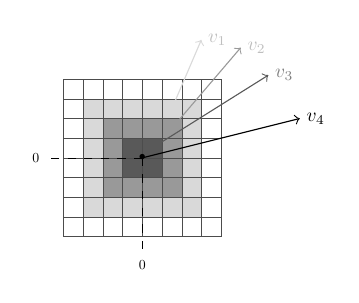
\begin{tikzpicture}[scale=0.5pt]                    
    \fill[thick,fill=gray!30] (-1.5, -1.5) -- (1.5, -1.5) -- (1.5, 1.5) -- (-1.5, 1.5);
    \fill[thick,fill=gray!80] (-1, -1) -- (1, -1) -- (1, 1) -- (-1, 1);
    \fill[thick,fill=gray!130] (-0.5, -0.5) -- (0.5, -0.5) -- (0.5, 0.5) -- (-0.5, 0.5);
    
    % Define the color and line thickness for easy reference
    \pgfkeys{/
      my/.style={
        line width=0.5pt,
      }
    }

    \foreach \x in {-2., -1.5, -1., -0.5, 0, 0.5, 1, 1.5, 2.} {
        \foreach \y in {-2., -1.5, -1, -0.5, 0, 0.5, 1., 1.5, 2.} {
            % Determine color based on the x coordinate
            \pgfmathsetmacro{\color}{(\x == 2 ? "white" : "black!70")}
                \draw[ultra thin, color=\color] (\x, \y) -- (\x + 0.5, \y);
            \pgfmathsetmacro{\color}{(\x == -2 ? "white" : "black!70")}
                \draw[ultra thin, color=\color] (\x, \y) -- (\x - 0.5, \y);                         
            \pgfmathsetmacro{\color}{(\y == 2 ? "white" : "black!70")}
                \draw[ultra thin, color=\color] (\x, \y) -- (\x , \y + 0.5);                            
            \pgfmathsetmacro{\color}{(\y == -2 ? "white" : "black!70")}
                \draw[ultra thin, color=\color] (\x, \y) -- (\x, \y - 0.5);

        }
    }

    \coordinate (a) at (0., 0);
    \coordinate (v) at (0., -2.5);
    \coordinate (h) at (-2.5, 0.);
    \draw[dashed, ultra thin, color=black](a)node{} -- (v)node[below, color=black, scale=0.5pt]{0};
    \draw[dashed, ultra thin, color=black](a)node{} -- (h)node[left, color=black, scale=0.5pt]{0};

    \coordinate (b) at (0. , 0.);
    \coordinate (b') at (4, 1.);
    \draw[->](b)node[scale=0.5pt]{$\bullet$}--(b')node[right, scale=0.7pt]{$v_4$};

    \coordinate (b) at (0.25 , 0.25);
    \coordinate (b') at (3.2, 2.1);
    \draw[->, color=gray!130](b)node{} -- (b')node[right, color=gray!100, scale=0.7pt]{$v_3$};

    \coordinate (b) at (0.75, 0.75);
    \coordinate (b') at (2.5, 2.8);
    \draw[->, color=gray!80](b)node{} -- (b')node[right, color=gray!50, scale=0.7pt]{$v_2$};

    \coordinate (b) at (0.75, 1.25);
    \coordinate (b') at (1.5, 3);
    \draw[->, color=gray!30](b)node{} -- (b')node[right, color=gray!50, scale=0.7pt]{$v_1$};
  \end{tikzpicture}
\end{center}